%%%%%%%%%%%%%%%%%%%%%%%%%%%%%%%%%%%%%%%%%%%%%%%%%%%%%%%%%%%%%%%%%%%%%%%%%%%%%%%%%
% Template: Exam
%
% Por: Abrantes Araújo Silva Filho
%      abrantesasf@gmail.com
%
% Citação: Se você gostou deste template, por favor ajude a divulgá-lo mantendo
%          o link para meu repositório GitHub em:
%          https://github.com/abrantesasf/LaTeX
%%%%%%%%%%%%%%%%%%%%%%%%%%%%%%%%%%%%%%%%%%%%%%%%%%%%%%%%%%%%%%%%%%%%%%%%%%%%%%%%%




%%%%%%%%%%%%%%%%%%%%%%%%%%%%%%%%%%%%%%%%%%%%%%%%%%%%%%%%%%%%%%%%%%%%%%%%%%%%%%%%%
%%% Configura o tipo de documento, papel, tamanho da fonte e informações básicas
%%% para as proriedades do PDF/DVIPS e outras propriedades do documento
\RequirePackage{ifpdf}
\ifpdf
  % Classe, língua e tamanho da fonte padrão. Outras opções a considerar:
  %   draft
  %   onecolumn (padrão) ou twocolumn (OU usar o package multicol)
  %   fleqn com ou sem leqno (alinhamento à esquerda das fórmulas e dos números)
  %   oneside (padrão para article ou report) ou twoside (padrão para book)
  %   answers = imprime respostas para o gabarito
  \documentclass[pdftex, brazil, 12pt, oneside, addpoints]{exam}
\else
  % Classe, língua e tamanho da fonte padrão. Outras opções a considerar:
  %   draft
  %   onecolumn (padrão) ou twocolumn (OU usar o package multicol)
  %   fleqn com ou sem leqno (alinhamento à esquerda das fórmulas e dos números)
  %   oneside (padrão para article ou report) ou twoside (padrão para book)
  %   answers = imprime respostas para o gabarito
  \documentclass[brazil, 12pt, oneside, addpoints]{exam}
\fi


%%%%%%%%%%%%%%%%%%%%%%%%%%%%%%%%%%%%%%%%%%%%%%%%%%%%%%%%%%%%%%%%%%%%%%%%%%%%%%%%%
%%% Carrega pacotes iniciais necessários para estrutura de controle e para a
%%% criação e o parse de novos comandos
\usepackage{ifthen}
\usepackage{xparse}


%%%%%%%%%%%%%%%%%%%%%%%%%%%%%%%%%%%%%%%%%%%%%%%%%%%%%%%%%%%%%%%%%%%%%%%%%%%%%%%%%
%%% Configuração do tamanho da página, margens, espaçamento entrelinhas e, se
%%% necessário, ativa a indentação dos primeiros parágrafos.
\ifpdf
  \usepackage[pdftex]{geometry}
\else
  \usepackage[dvips]{geometry}
\fi
\geometry{a4paper, left=2.0cm, right=2.0cm, top=2.0cm, bottom=2.0cm}

\usepackage{setspace}
  \singlespacing
  %\onehalfspacing
  %\doublespacing


%%%%%%%%%%%%%%%%%%%%%%%%%%%%%%%%%%%%%%%%%%%%%%%%%%%%%%%%%%%%%%%%%%%%%%%%%%%%%%%%%
%%% Configurações de encoding, lingua e fontes:
\usepackage[T1]{fontenc}
\usepackage[utf8]{inputenc}
\usepackage{babel}

% Altera a fonte padrão do documento (nem todas funcionam em modo math):
%   phv = Helvetica
%   ptm = Times
%   ppl = Palatino
%   pbk = bookman
%   pag = AdobeAvantGarde
%   pnc = Adobe NewCenturySchoolBook
\renewcommand{\familydefault}{ppl}


%%%%%%%%%%%%%%%%%%%%%%%%%%%%%%%%%%%%%%%%%%%%%%%%%%%%%%%%%%%%%%%%%%%%%%%%%%%%%%%%%
%%% Configurações de cabeçalho e rodapé (não pode usar fancyhdr pois ocorre conflito):
\pagestyle{headandfoot}
\runningheadrule
\firstpageheader{}{}{}
\runningheader{Exercício 1: conceitos básicos}{}{Setembro/2019}
\firstpagefooter{}{}{Página \thepage\ de \numpages}
\runningfooter{}{}{Página \thepage\ de \numpages}
\runningfootrule


%%%%%%%%%%%%%%%%%%%%%%%%%%%%%%%%%%%%%%%%%%%%%%%%%%%%%%%%%%%%%%%%%%%%%%%%%%%%%%%%%
%%% Carrega bibliotecas de símbolos (matemáticos, físicos, etc.), fontes
%%% adicionais, e configura algumas opções
\usepackage{amsmath}
\usepackage{amssymb}
\usepackage{amsfonts}
\usepackage{siunitx}
  \sisetup{group-separator = {.}}
  \sisetup{group-digits = {false}}
  \sisetup{output-decimal-marker = {,}}
\usepackage{bm}
\usepackage{cancel}
% Altera separador decimal via comando, se necessário (prefira o siunitx):
%\mathchardef\period=\mathcode`.
%\DeclareMathSymbol{.}{\mathord}{letters}{"3B}


%%%%%%%%%%%%%%%%%%%%%%%%%%%%%%%%%%%%%%%%%%%%%%%%%%%%%%%%%%%%%%%%%%%%%%%%%%%%%%%%%
%%% Carrega pacotes para referências cruzadas, citações dentro do documento,
%%% links para internet e outros.Configura algumas opções.
%%% Não altere a ordem de carregamento dos packages.
\usepackage{varioref}
\ifpdf
  \usepackage[pdftex]{hyperref}
    \hypersetup{
      % Informações variáveis em cada documento (MUDE AQUI!):
      pdftitle={Exercício 1: conceitos básicos sobre matrizes},
      pdfauthor={Abrantes Araújo Silva Filho},
      pdfsubject={Matrizes},
      pdfkeywords={matrizes, conceitos},
      pdfinfo={
        CreationDate={}, % Ex.: D:AAAAMMDDHH24MISS
        ModDate={}       % Ex.: D:AAAAMMDDHH24MISS
      },
      % Coisas que você não deve alterar se não souber o que está fazendo:
      unicode=true,
      pdflang={pt-BR},
      bookmarksopen=true,
      bookmarksnumbered=true,
      bookmarksopenlevel=5,
      pdfdisplaydoctitle=true,
      pdfpagemode=UseOutlines,
      pdfstartview=FitH,
      pdfcreator={LaTeX with hyperref package},
      pdfproducer={pdfTeX},
      pdfnewwindow=true,
      colorlinks=true,
      citecolor=green,
      linkcolor=red,
      filecolor=cyan,
      urlcolor=blue
    }
\else
  \usepackage{hyperref}
\fi
\usepackage{cleveref}
\usepackage{url}
  

%%%%%%%%%%%%%%%%%%%%%%%%%%%%%%%%%%%%%%%%%%%%%%%%%%%%%%%%%%%%%%%%%%%%%%%%%%%%%%%%%
%%% Carrega packages relacionados à computação
\usepackage{algorithm2e}
\usepackage{algorithmicx}
\usepackage{algpseudocode}
\usepackage{listings}
  \lstset{literate=
    {á}{{\'a}}1 {é}{{\'e}}1 {í}{{\'i}}1 {ó}{{\'o}}1 {ú}{{\'u}}1
    {Á}{{\'A}}1 {É}{{\'E}}1 {Í}{{\'I}}1 {Ó}{{\'O}}1 {Ú}{{\'U}}1
    {à}{{\`a}}1 {è}{{\`e}}1 {ì}{{\`i}}1 {ò}{{\`o}}1 {ù}{{\`u}}1
    {À}{{\`A}}1 {È}{{\'E}}1 {Ì}{{\`I}}1 {Ò}{{\`O}}1 {Ù}{{\`U}}1
    {ä}{{\"a}}1 {ë}{{\"e}}1 {ï}{{\"i}}1 {ö}{{\"o}}1 {ü}{{\"u}}1
    {Ä}{{\"A}}1 {Ë}{{\"E}}1 {Ï}{{\"I}}1 {Ö}{{\"O}}1 {Ü}{{\"U}}1
    {â}{{\^a}}1 {ê}{{\^e}}1 {î}{{\^i}}1 {ô}{{\^o}}1 {û}{{\^u}}1
    {Â}{{\^A}}1 {Ê}{{\^E}}1 {Î}{{\^I}}1 {Ô}{{\^O}}1 {Û}{{\^U}}1
    {œ}{{\oe}}1 {Œ}{{\OE}}1 {æ}{{\ae}}1 {Æ}{{\AE}}1 {ß}{{\ss}}1
    {ű}{{\H{u}}}1 {Ű}{{\H{U}}}1 {ő}{{\H{o}}}1 {Ő}{{\H{O}}}1
    {ç}{{\c c}}1 {Ç}{{\c C}}1 {ø}{{\o}}1 {å}{{\r a}}1 {Å}{{\r A}}1
    {€}{{\euro}}1 {£}{{\pounds}}1 {«}{{\guillemotleft}}1
    {»}{{\guillemotright}}1 {ñ}{{\~n}}1 {Ñ}{{\~N}}1 {¿}{{?`}}1
  }
  

%%%%%%%%%%%%%%%%%%%%%%%%%%%%%%%%%%%%%%%%%%%%%%%%%%%%%%%%%%%%%%%%%%%%%%%%%%%%%%%%%
%%% Ativa suporte extendido a cores
\usepackage[svgnames]{xcolor} % Opções de cores: usenames (16), dvipsnames (64),
                              % svgnames (150) e x11names (300).


%%%%%%%%%%%%%%%%%%%%%%%%%%%%%%%%%%%%%%%%%%%%%%%%%%%%%%%%%%%%%%%%%%%%%%%%%%%%%%%%%
%%% Suporte à importação de gráficos externos
\ifpdf
  \usepackage[pdftex]{graphicx}
\else
  \usepackage[dvips]{graphicx}
\fi


%%%%%%%%%%%%%%%%%%%%%%%%%%%%%%%%%%%%%%%%%%%%%%%%%%%%%%%%%%%%%%%%%%%%%%%%%%%%%%%%%
%%% Suporte à criação de gráficos proceduralmente na LaTeX:
\usepackage{tikz}
  \usetikzlibrary{arrows,automata,backgrounds,matrix,patterns,positioning,shapes,shadows}


%%%%%%%%%%%%%%%%%%%%%%%%%%%%%%%%%%%%%%%%%%%%%%%%%%%%%%%%%%%%%%%%%%%%%%%%%%%%%%%%%
%%% Packages para tabelas
\usepackage{array}
\usepackage{longtable}
\usepackage{tabularx}
\usepackage{tabu}
\usepackage{lscape}
\usepackage{colortbl}  
\usepackage{booktabs}
\newcolumntype{M}[1]{>{\centering\arraybackslash}m{#1}}
%\newcolumntype{ML}[1]{>{$}l<{$}}
%\newcolumntype{MR}[1]{>{R}r<{R}}
\newcolumntype{L}[1]{>{\arraybackslash}m{#1}}
\newcolumntype{N}{@{}m{0pt}@{}}


%%%%%%%%%%%%%%%%%%%%%%%%%%%%%%%%%%%%%%%%%%%%%%%%%%%%%%%%%%%%%%%%%%%%%%%%%%%%%%%%%
%%% Packages ambientes de listas
\usepackage{enumitem}
\usepackage[ampersand]{easylist}


%%%%%%%%%%%%%%%%%%%%%%%%%%%%%%%%%%%%%%%%%%%%%%%%%%%%%%%%%%%%%%%%%%%%%%%%%%%%%%%%%
%%% Packages para suporte a ambientes floats, captions, etc.:
\usepackage{float}
\usepackage{wrapfig}
\usepackage{placeins}
\usepackage{caption}
\usepackage{sidecap}
\usepackage{subcaption}


%%%%%%%%%%%%%%%%%%%%%%%%%%%%%%%%%%%%%%%%%%%%%%%%%%%%%%%%%%%%%%%%%%%%%%%%%%%%%%%%%
%%% Meus comandos específicos:
% Commando para ``italizar´´ palavras em inglês (e outras línguas!):
\newcommand{\ingles}[1]{\textit{#1}}

% Commando para colocar o espaço correto entre um número e sua unidade:
\newcommand{\unidade}[2]{\ensuremath{#1\,\mathrm{#2}}}
\newcommand{\unidado}[2]{{#1}\,{#2}}

% Produz ordinal masculino ou feminino dependendo do segundo argumento:
\newcommand{\ordinal}[2]{%
#1%
\ifthenelse{\equal{a}{#2}}%
{\textordfeminine}%
{\textordmasculine}}


%%%%%%%%%%%%%%%%%%%%%%%%%%%%%%%%%%%%%%%%%%%%%%%%%%%%%%%%%%%%%%%%%%%%%%%%%%%%%%%%%
%%% Hifenização específica quando o LaTeX/Babel não conseguirem hifenizar:
\babelhyphenation{Git-Hub}


%%%%%%%%%%%%%%%%%%%%%%%%%%%%%%%%%%%%%%%%%%%%%%%%%%%%%%%%%%%%%%%%%%%%%%%%%%%%%%%%%
%%% Comandos específicos para a classe EXAM deste documento:
\newcommand{\umalinha}{\fillwithlines{0.25in}}
\newcommand{\duaslinhas}{\fillwithlines{0.50in}}
\newcommand{\treslinhas}{\fillwithlines{0.75in}}
\newcommand{\quatrolinhas}{\fillwithlines{1.00in}}
\newcommand{\cincolinhas}{\fillwithlines{1.25in}}
\newcommand{\seislinhas}{\fillwithlines{1.50in}}
\newcommand{\setelinhas}{\fillwithlines{1.75in}}
\newcommand{\oitolinhas}{\fillwithlines{2.00in}}
\newcommand{\novelinhas}{\fillwithlines{2.25in}}
\newcommand{\dezlinhas}{\fillwithlines{2.50in}}

% Verdadeiro ou Falvo para a classe EXAM
\newcommand{\vf}[1][{}]{%
  \fillin[#1][0.25in]%
}

% Título das respostas:
%\renewcommand{\solutiontitle}{\noindent\textbf{Resposta:}\par\noindent}
\renewcommand{\solutiontitle}{\noindent}
%\shadedsolutions
%\SolutionEmphasis{\itshape}




%%%%%%%%%%%%%%%%%%%%%%%%%%%%%%%%%%%%%%%%%%%%%%%%%%%%%%%%%%%%%%%%%%%%%%%%%%%%%%%%%
%%%%%%%%%%%%%%%%%%%%%%%%%%%%%%%%%%%%%%%%%%%%%%%%%%%%%%%%%%%%%%%%%%%%%%%%%%%%%%%%%
%%%%%%%%%%%%%%%%%%%%%%%%%%%%%%%%%%%%%%%%%%%%%%%%%%%%%%%%%%%%%%%%%%%%%%%%%%%%%%%%%
%%%%%%%%%%%%%%%%%%%%%%%%%%%%%%%%%%%%%%%%%%%%%%%%%%%%%%%%%%%%%%%%%%%%%%%%%%%%%%%%%
%%%%%%%%%%%%%%%%%%%%%%%%%%%%%% COMEÇA O DOCUMENTO %%%%%%%%%%%%%%%%%%%%%%%%%%%%%%%
%%%%%%%%%%%%%%%%%%%%%%%%%%%%%%%%%%%%%%%%%%%%%%%%%%%%%%%%%%%%%%%%%%%%%%%%%%%%%%%%%
%%%%%%%%%%%%%%%%%%%%%%%%%%%%%%%%%%%%%%%%%%%%%%%%%%%%%%%%%%%%%%%%%%%%%%%%%%%%%%%%%
%%%%%%%%%%%%%%%%%%%%%%%%%%%%%%%%%%%%%%%%%%%%%%%%%%%%%%%%%%%%%%%%%%%%%%%%%%%%%%%%%
%%%%%%%%%%%%%%%%%%%%%%%%%%%%%%%%%%%%%%%%%%%%%%%%%%%%%%%%%%%%%%%%%%%%%%%%%%%%%%%%%
\begin{document}


%%%%%%%%%%%%%%%%%%%%%%%%%%%%%%%%%%%%%%%%%%%%%%%%%%%%%%%%%%%%%%%%%%%%%%%%%%%%%%%%%
%%%%%%%%%%%%%%%%%%%%%%%%%%%%%%%%%%%%%%%%%%%%%%%%%%%%%%%%%%%%%%%%%%%%%%%%%%%%%%%%%
%%%%%%%%%%%%%%%%%%%%%%%%%%%%%%%%%%%%%%%%%%%%%%%%%%%%%%%%%%%%%%%%%%%%%%%%%%%%%%%%%
\begin{coverpages}

\begin{center}
\textbf{\textit{\Large%
Álgebra Linear\\
--- monitoria ---}}
\end{center}

\vspace{1cm}

\begin{figure}[H]
\begin{center}
\fbox{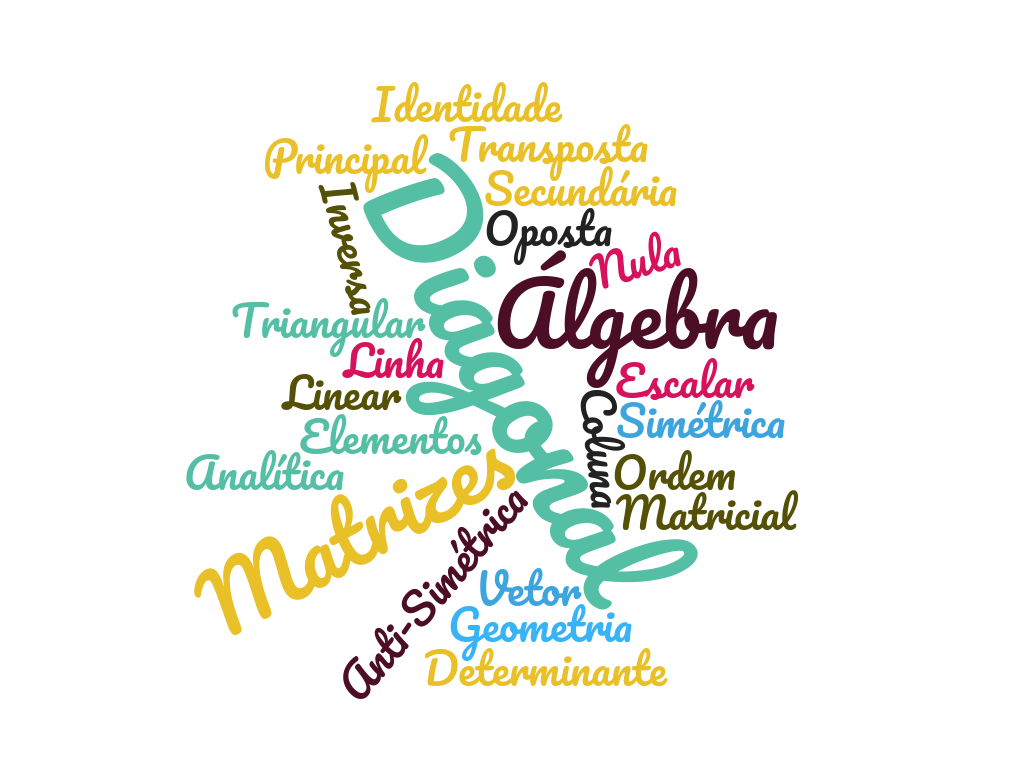
\includegraphics[scale=0.4]{linear_algebra.png}}
\end{center}
\end{figure}

\vspace{1cm}

\begin{center}
\textit{\textbf{\Large%
--- Exercício 1: conceitos sobre matrizes ---\\
\ \\
Setembro/2019}}
\end{center}

%\vspace{1cm}
%\begin{flushright}
%\textbf{Monitor(es):}\\
%\textit{Monitor 1\\
%Monitor 2}
%\end{flushright}

%\begin{center}
%  \fbox{\fbox{\parbox{5.5in}{\centering
%        Answer the questions in the spaces provided on the
%        question sheets. If you run out of room for an answer,
%        continue on the back of the page.}}}
%\end{center}

\end{coverpages}

\newpage

\begin{questions}
\setlength\linefillthickness{0.2pt}
%%%%%%%%%%%%%%%%%%%%%%%%%%%%%%%%%%%%%%%%%%%%%%%%%%%%%%%%%%%%%%%%%%%%%%%%%%%%%%%%%
%%%%%%%%%%%%%%%%%%%%%%%%%%%%%%%%%%%%%%%%%%%%%%%%%%%%%%%%%%%%%%%%%%%%%%%%%%%%%%%%%
%%%%%%%%%%%%%%%%%%%%%%%%%%%%%%%%%%%%%%%%%%%%%%%%%%%%%%%%%%%%%%%%%%%%%%%%%%%%%%%%%
\fullwidth{\section{Conceitos básicos sobre matrizes}}
%\ifprintanswers
%\newpage
%\else
%\newpage
%\fi

\question
De forma geral, o que é uma matriz?
\begin{solutionorlines}[0.50in]
  É um quadro retangular de números dispostos em linhas e colunas.
\end{solutionorlines}

\question
Indique se a sentença é verdadeira (V) ou falsa (F):
\begin{parts}
  \part \vf[F] Em geral, as matrizes são identificadas por letras minúsculas
  \part \vf[F] As matrizes só podem ser delimitadas por parênteses ou colchetes
  \part \vf[V] A representação ``$A = [-3]$'' indica uma matriz chamada $A$ que contém
  um único elemento, $-3$.
  \part \vf[V] Os números que formam a matriz são chamados de elementos.
  \part \vf[F] A seguinte matriz é uma matriz coluna: $C = [3\quad 4\quad 5]$
\end{parts}

\question
O que é a \emph{ordem} (ou \emph{tipo}) de uma matriz? Como a \emph{ordem} é
representada?
\begin{solutionorlines}[0.75in]
  A \emph{ordem} de uma matriz indica a quantidade de linhas e colunas que a matriz
  tem. É representada por $m \times n$, onde $m$ indica a quantidade de \emph{linhas}
  e $n$ indica a quantidade de \emph{colunas}.
\end{solutionorlines}

\question
Qual a ordem da matriz
$A = \begin{pmatrix}
a & b & c\\
d & e & f\end{pmatrix}$? E o tipo da matriz
$B = \begin{pmatrix}
  1 & -3 & 0 & 7 & 2\\
  2 & -2 & 4 & 5 & \sqrt{3}\\
  3 & -1 & 6 & 3 & 9
\end{pmatrix}$?
\begin{solutionorlines}[0.50in]
  A matriz A é da ordem $2 \times 3$, e a matriz B é da ordem $3 \times 5$.
\end{solutionorlines}

\question
O que é uma matriz \emph{quadrada} de ordem $n$?
\begin{solutionorlines}[0.50in]
  É uma matriz na qual o número de linhas é igual ao número de colunas, ou seja,
  tem a ordem $m \times n,\ m = n$.
\end{solutionorlines}

\question
Em uma matriz quadrada A de ordem $n$, podemos afirmar que sua \emph{diagonal
  principal} é formada pelos elementos $a_{11}, a_{22}, a_{33}, \cdots, a_{nn}$? Por quê?
\begin{solutionorlines}[0.75in]
  Sim, pois se a matriz é quadrada sua diagonal principal será formada por todos os
  elementos nos quais $m = n$, ou seja, $a_{11}, a_{22}, a_{33}, \cdots, a_{nn}$.

  Por exemplo: se B é uma matriz quadrada de ordem 3, sua diagonal principal é:

  $B = \begin{pmatrix}
   \color{red} b_{11} & b_{12} & b_{13}\\
   b_{21} & \color{red} b_{22} & b_{23}\\
   b_{31} & b_{32} & \color{red} b_{33}
  \end{pmatrix}$ 
\end{solutionorlines}

\question
Indique se a sentença é verdadeira (V) ou falsa (F):
\begin{parts}
  \part \vf[F] Matrizes que não são quadradas, não têm diagonal principal
  \part \vf[F] Matrizes que não são quadradas, não têm diagonal secundária
  \part \vf[V] Toda matriz tem uma, e somente uma, diagonal principal
  \part \vf[V] Toda matriz tem uma, e somente uma, diagonal secundária
  \part \vf[F] Matriz quadrada de ordem $n$ não têm diagonal secundária
  \part \vf[V] Os elementos formados pelos números ``1'' na matriz $E = \begin{pmatrix}
   \color{red} 1 & 0 & 0 & 0\\
   0 & \color{red} 1 & 0 & 0\\
   0 & 0 & \color{red} 1 & 0\end{pmatrix}$, representam sua diagonal principal
  \part \vf[F] Os elementos formados pelos números ``1'' na matriz $F = \begin{pmatrix}
    0 & 0 & 0 & \color{red} 1\\
   0 & 0 & \color{red} 1 & 0\\
   0 & \color{red} 1 & 0 & 0\end{pmatrix}$, representam sua diagonal principal
  \part \vf[V] Uma matriz com ordem $1 \times n$ é uma matriz linha
  \part \vf[V] Uma matriz com ordem $m \times 1$ é uma matriz coluna
  \part \vf[F] Uma matriz com ordem $7 \times 5$ tem 75 elementos
  \part \vf[V] Em uma matriz quadrada de ordem $n$, os elementos tais que
  $i + j = n + 1$ formam a diagonal secundária
\end{parts}

\question
A representação da seguinte matriz está correta? Por quê?

$A = \begin{Vmatrix}
  -1 & 7 & 2\\
  0 & 5 & -5\end{Vmatrix}_{3 \times 2}$
\begin{solutionorlines}[0.50in]
  Não, pois a matriz não é do tipo $3 \times 2$, e sim do tipo
  $2 \times 3$.
\end{solutionorlines}

\question
O que significa dizer que uma determinada matriz tem 2 elementos nulos?
\begin{solutionorlines}[0.50in]
  Que 2 de seus elementos são $0$.
\end{solutionorlines}

\question
Uma matriz $A$ pode ser representada pela notação $A = (a_{ij})_{m \times n}$
onde $a_{ij}$ ou $[A]_{ij}$ é o elemento na linha $i$ e coluna $j$ dessa
matriz. Em relação a essa forma de notação, marque a resposta correta:
\begin{checkboxes}
  \choice Se uma matriz $B$ tem ordem $3 \times 2$, o elemento $b_{42}$ estará
  localizado em alguma das diagonais da matriz (principal ou secundária)
  \choice Uma matriz $C$ com ordem $4 \times 2$ não pode ter um elemento
  na posição $c_{31}$
  \choice Não existe como indicar todos os elementos da j-ésima coluna de uma matriz
  \CorrectChoice A i-ésima linha de uma matriz $A$ qualquer, com ordem $m \times n$, corresponde aos
  elementos $a_{i1}, a_{i2}, a_{i3}, \cdots, a_{in}$
  \choice A j-ésima linha de uma matriz $A$ qualquer, com ordem $m \times n$, corresponde aos
  elementos $a_{1j}, a_{2j}, a_{3j}, \cdots, a_{mj}$
\end{checkboxes}

\ifprintanswers
\newpage
\else
\newpage
\fi

\question
Sabendo-se que uma matriz qualquer $A$ de ordem $m \times n$ tem a forma
genérica

$A = \begin{pmatrix}
  a_{11} & a_{12} & a_{13} & \cdots & a_{1n}\\
  a_{21} & a_{22} & a_{23} & \cdots & a_{2n}\\
  \vdots & \vdots & \vdots & \ddots & \vdots\\
  a_{m1} & a_{m2} & a_{m3} & \cdots & a_{mn}\\
\end{pmatrix}$,

construa a matriz $B = (b_{ij})_{5 \times 4}$, onde
%\begin{equation}
$b_{ij} =
    \begin{cases}
      i \times j & \text{se}\ i < j\\
      j \div i   & \text{se}\ i > j\\
      i + j      & \text{se}\ i = j
    \end{cases}
$
%\end{equation}
\begin{solutionorbox}[1.5in]
$B = \begin{pmatrix}
   2    & 2    & 3    & 4\\
   1/2  & 4    & 6    & 8\\
   1/3  & 2/3  & 6    & 12\\
   1/4  & 2/4  & 3/4  & 8\\
   1/5  & 2/5  & 3/5  & 4/5\\
\end{pmatrix}$
\end{solutionorbox}


%%%%%%%%%%%%%%%%%%%%%%%%%%%%%%%%%%%%%%%%%%%%%%%%%%%%%%%%%%%%%%%%%%%%%%%%%%%%%%%%%
%%%%%%%%%%%%%%%%%%%%%%%%%%%%%%%%%%%%%%%%%%%%%%%%%%%%%%%%%%%%%%%%%%%%%%%%%%%%%%%%%
%%%%%%%%%%%%%%%%%%%%%%%%%%%%%%%%%%%%%%%%%%%%%%%%%%%%%%%%%%%%%%%%%%%%%%%%%%%%%%%%%
\fullwidth{\section{Matrizes especiais}}

\question
Já vimos e estudamos 12 (doze) tipos de matrizes especiais, ou seja, aquelas matrizes
que apresentam alguma particularidade que as diferenciam de outras matrizes genéricas.
Liste todas as matrizes especiais:
\ifprintanswers
\begin{solution}
  \vspace{-0.7cm}
\begin{enumerate}
  \item Matriz Quadrada
  \item Matriz Linha
  \item Matriz Coluna
  \item Matriz Nula
  \item Matriz Diagonal
  \item Matriz Triangular
  \item Matriz Identidade
  \item Matriz Transposta
  \item Matriz Oposta
  \item Matriz Simétrica
  \item Matriz Anti-Simétrica
  \item Matriz Inversa
\end{enumerate}
\end{solution}
\else
\begin{enumerate}
  \item \_\_\_\_\_\_\_\_\_\_\_\_\_\_\_\_\_\_\_\_\_\_\_\_\_\_\_\_\_\_\_\_\_\_\_\_\_\_\_\_\_\_\_\_\_\_\_\_\_\_\_\_\_\_\_\_
  \item \_\_\_\_\_\_\_\_\_\_\_\_\_\_\_\_\_\_\_\_\_\_\_\_\_\_\_\_\_\_\_\_\_\_\_\_\_\_\_\_\_\_\_\_\_\_\_\_\_\_\_\_\_\_\_\_
  \item \_\_\_\_\_\_\_\_\_\_\_\_\_\_\_\_\_\_\_\_\_\_\_\_\_\_\_\_\_\_\_\_\_\_\_\_\_\_\_\_\_\_\_\_\_\_\_\_\_\_\_\_\_\_\_\_
  \item \_\_\_\_\_\_\_\_\_\_\_\_\_\_\_\_\_\_\_\_\_\_\_\_\_\_\_\_\_\_\_\_\_\_\_\_\_\_\_\_\_\_\_\_\_\_\_\_\_\_\_\_\_\_\_\_
  \item \_\_\_\_\_\_\_\_\_\_\_\_\_\_\_\_\_\_\_\_\_\_\_\_\_\_\_\_\_\_\_\_\_\_\_\_\_\_\_\_\_\_\_\_\_\_\_\_\_\_\_\_\_\_\_\_
  \item \_\_\_\_\_\_\_\_\_\_\_\_\_\_\_\_\_\_\_\_\_\_\_\_\_\_\_\_\_\_\_\_\_\_\_\_\_\_\_\_\_\_\_\_\_\_\_\_\_\_\_\_\_\_\_\_
  \item \_\_\_\_\_\_\_\_\_\_\_\_\_\_\_\_\_\_\_\_\_\_\_\_\_\_\_\_\_\_\_\_\_\_\_\_\_\_\_\_\_\_\_\_\_\_\_\_\_\_\_\_\_\_\_\_
  \item \_\_\_\_\_\_\_\_\_\_\_\_\_\_\_\_\_\_\_\_\_\_\_\_\_\_\_\_\_\_\_\_\_\_\_\_\_\_\_\_\_\_\_\_\_\_\_\_\_\_\_\_\_\_\_\_
  \item \_\_\_\_\_\_\_\_\_\_\_\_\_\_\_\_\_\_\_\_\_\_\_\_\_\_\_\_\_\_\_\_\_\_\_\_\_\_\_\_\_\_\_\_\_\_\_\_\_\_\_\_\_\_\_\_
  \item \_\_\_\_\_\_\_\_\_\_\_\_\_\_\_\_\_\_\_\_\_\_\_\_\_\_\_\_\_\_\_\_\_\_\_\_\_\_\_\_\_\_\_\_\_\_\_\_\_\_\_\_\_\_\_\_
  \item \_\_\_\_\_\_\_\_\_\_\_\_\_\_\_\_\_\_\_\_\_\_\_\_\_\_\_\_\_\_\_\_\_\_\_\_\_\_\_\_\_\_\_\_\_\_\_\_\_\_\_\_\_\_\_\_
  \item \_\_\_\_\_\_\_\_\_\_\_\_\_\_\_\_\_\_\_\_\_\_\_\_\_\_\_\_\_\_\_\_\_\_\_\_\_\_\_\_\_\_\_\_\_\_\_\_\_\_\_\_\_\_\_\_    
\end{enumerate}
\fi

\ifprintanswers
\newpage
\fi

\question
O que é uma \emph{matriz nula}? Que letra geralmente é utilizada para representar tal matriz?
\begin{solutionorlines}[0.50in]
  É uma matriz na qual todos os seus elementos são nulos, ou seja, são zeros. É geralmente
  representada pela letra $O$. Por exemplo, uma matriz $O_{2 \times 3}$ é a matriz nula
  de ordem $2 \times 3$.
\end{solutionorlines}

\question
A matriz nula $O = (0)$ é uma matriz quadrada, uma matriz linha ou uma matriz coluna?
\begin{solutionorlines}[0.50in]
  Essa matriz pode ser considerada tudo isso ao mesmo tempo pois sua ordem é $1 \times 1$
  (e portanto é quadrada), tem apenas 1 linha (e portanto é uma matriz linha) e tem apenas
  1 coluna (e portanto é uma matriz coluna).
\end{solutionorlines}

\question
O que é uma \emph{matriz diagonal}?
\begin{solutionorlines}[0.50in]
  É uma matriz \emph{quadrada} na qual todos os elementos que \emph{não estão}
  na diagonal principal são nulos.
\end{solutionorlines}

\question
O que é uma \emph{matriz triangular}?
\begin{solutionorlines}[0.50in]
  É uma matriz \emph{quadrada} na qual todos os elementos que \emph{estão acima}
  OU que \emph{estão abaixo} da diagonal principal são nulos.
\end{solutionorlines}

\question
Indique se a sentença é verdadeira (V) ou falsa (F):
\begin{parts}
  \part \vf[F] Em situações especiais, como na multiplicação de matrizes,
  uma matriz nula pode conter um elemento com o valor 1
  \part \vf[F] Uma matriz retangular de ordem $m \times n$ com $m \ne n$ não pode ser nula
  \part \vf[F] Uma matriz diagonal é uma matriz retangular de ordem $m \times n$ com $m \ne n$,
  na qual todos os elementos que não estão na diagonal principal são nulos
  \part \vf[V] Uma matriz diagonal pode ter a diagonal principal com todos os elementos nulos
  \part \vf[F] Uma matriz triangular de ordem $n$ é aquela onde todos os elementos que estão
  acima da diagonal principal, E MAIS todos os elementos que estão abaixo da diagonal principal, são nulos.
  \part \vf[V] Para que uma matriz seja considerada triangular, todos os elementos que estão acima OU abaixo
  da diagonal principal (não simultaneamente) devem ser nulos.
  \part \vf[F] Uma matriz diagonal nunca poderá ser uma matriz nula
\end{parts}

\ifprintanswers
\newpage
\fi

\question
O que é uma \emph{matriz identidade}? Que letra geralmente é utilizada para representar
tal matriz?
\begin{solutionorlines}[0.50in]
  É uma matriz diagonal na qual todos os elementos da \emph{diagonal principal}
  são unitários, ou seja, são o valor 1. É geralmente representada pela letra $I$.
\end{solutionorlines}

\question
O que é uma \emph{matriz transposta}? Como é representada?
\begin{solutionorlines}[0.50in]
  É aquela na qual as linhas de uma matriz passam a ser as colunas da outra, e é
  representada pela letra ``t'' sobrescrita, por exemplo: $A^t$ é a matriz
  transposta de $A$.

  Mais especificamente, a transposta de uma matriz $A$ de ordem $m \times n$, é a
  matriz $A^t$ de ordem $n \times m$ tal que as linhas da matriz $A$ passam a er
  as colunas ma matriz $A^t$.
\end{solutionorlines}

\question
Indique se a sentença é verdadeira (V) ou falsa (F):
\begin{parts}
  \part \vf[F] Uma matriz nula $O$ de ordem 1 pode ser uma matriz identidade
  \part \vf[F] Uma matriz identidade não precisa ser quadrada
  \part \vf[F] A diagonal secundária de uma matriz identidade tem todos os seus
  elementos nulos
  \part \vf[V] A diagonal principal de uma matriz identidade tem todos os seus
  elementos unitários
  \part \vf[V] Existe uma matriz identidade de ordem 1, ou seja, $I_1 = [1]$
  \part \vf[F] Para que uma matriz $A$ seja transposta em $A^t$, é necessário
  que ela seja quadrada
  \part \vf[F] Dada uma matriz identidade $I$ qualquer, sua transposta $I^t$ não é
  mais uma matriz identidade
  \part \vf[F] A transposta de uma matriz nula $O$ de ordem $m \times n$ com $m \ne n$,
  também será uma matriz nula $O^t$ com a mesma ordem
  \part \vf[V] A matriz transposta $B^t$ de uma matriz $B$ só terá a mesma ordem
  da matriz $B$ se a matriz $B$ for quadrada
  \part \vf[V] $(A^t)^t = A$
\end{parts}

\question
O que é uma \emph{matriz oposta}? Como é representada?
\begin{solutionorlines}[0.50in]
  É uma matriz que foi multiplicada por $-1$, ou seja, teve todos os seus
  elementos multiplicados por $-1$. É representada por um menos unário no
  nome da matriz, por exemplo, a matriz $-C$ é a oposta da matriz $C$.
\end{solutionorlines}

\question
O que é uma \emph{matriz simétrica}?
\begin{solutionorlines}[0.50in]
  É uma matriz que é idêntica à sua transposta, ou seja, uma matriz $B$
  é simétrica se $B = B^t$.
\end{solutionorlines}

\question
Uma matriz de ordem $m \times n$ com $m \ne n$ pode ser simétrica? Por quê?
\begin{solutionorlines}[0.50in]
  Não, pois a ordem da transposta não seria igual à ordem da matriz original e
  isso indica que a matriz original não é idêntica à sua transposta.
\end{solutionorlines}

\question
O que é uma \emph{matriz anti-simétrica}?
\begin{solutionorlines}[0.50in]
  É uma matriz que é idêntica à oposta de sua transposta, ou seja, uma matriz $B$
  é anti-simétrica se $B = -(B^t)$.
\end{solutionorlines}

\question
Marque a(s) alternativa(s) que corresponde(m) à seguinte matriz:

\hspace{5cm}$B = \begin{pmatrix}
  0 & 0 & 0\\
  0 & 0 & 0\\
  0 & 0 & 0
\end{pmatrix}$
\begin{checkboxes}
  \choice Matriz Identidade
  \CorrectChoice Matriz Nula
  \choice Matriz Coluna
  \CorrectChoice Matriz Diagonal
  \choice Matriz Triangular
\end{checkboxes}

\question
Marque a(s) alternativa(s) que corresponde(m) à seguinte matriz:

\hspace{5cm}$D = \begin{pmatrix}
  7
\end{pmatrix}$
\begin{checkboxes}
  \choice Matriz Identidade
  \CorrectChoice Matriz Quadrada
  \choice Matriz Nula
  \CorrectChoice Matriz Linha
  \CorrectChoice Matriz Coluna
\end{checkboxes}

\question
Marque a(s) alternativa(s) que corresponde(m) à seguinte matriz:

\hspace{5cm}$E = \begin{pmatrix}
  1 & 0 & 0\\
  0 & 1 & 0\\
  0 & 0 & 0
\end{pmatrix}$
\begin{checkboxes}
  \CorrectChoice Matriz Diagonal
  \CorrectChoice Matriz Simétrica
  \choice Matriz Anti-Simétrica
  \choice Matriz Triangular
  \choice Matriz Identidade
\end{checkboxes}

\ifprintanswers
\newpage
\fi

\question
Marque a(s) alternativa(s) que corresponde(m) à seguinte matriz:

\hspace{5cm}$F = \begin{pmatrix}
  0 & 0 & 1\\
  0 & 1 & 0\\
  1 & 0 & 0
\end{pmatrix}$
\begin{checkboxes}
  \choice Matriz Identidade
  \choice Matriz Triangular
  \choice Matriz Diagonal
  \CorrectChoice Matriz Simétrica
  \choice Matriz Nula
\end{checkboxes}

\question
Marque a(s) alternativa(s) que corresponde(m) à seguinte matriz:

\hspace{5cm}$G = \begin{pmatrix}
  0 & -2 & 0\\
  2 & 0 & 3\\
  0 & -3 & 0
\end{pmatrix}$
\begin{checkboxes}
  \choice Matriz Identidade
  \choice Matriz Triangular
  \choice Matriz Diagonal
  \CorrectChoice Matriz Anti-Simétrica
  \choice Nenhuma das respostas acima
\end{checkboxes}

\question
Indique se a sentença é verdadeira (V) ou falsa (F):
\begin{parts}
  \part \vf[V] Existe uma matriz nula, quadrada, linha, coluna, diagonal, simétrica e anti-simétrica
  \part \vf[F] Existe uma matriz nula, diagonal e triangular
  \part \vf[V] Toda matriz anti-simétrica tem sua diagonal principal composta por elementos nulos (zeros)
  \part \vf[V] Se $A = -1B$, então $B$ é a oposta de $A$
  \part \vf[F] Se $A = A^t$, então elas não são simétricas
  \part \vf[V] Se $B = -(B^t)$, então elas são anti-simétricas
  \part \vf[F] $A \ne (A^t)^t$
\end{parts}


%%%%%%%%%%%%%%%%%%%%%%%%%%%%%%%%%%%%%%%%%%%%%%%%%%%%%%%%%%%%%%%%%%%%%%%%%%%%%%%%%
%%%%%%%%%%%%%%%%%%%%%%%%%%%%%%%%%%%%%%%%%%%%%%%%%%%%%%%%%%%%%%%%%%%%%%%%%%%%%%%%%
%%%%%%%%%%%%%%%%%%%%%%%%%%%%%%%%%%%%%%%%%%%%%%%%%%%%%%%%%%%%%%%%%%%%%%%%%%%%%%%%%
\fullwidth{\section{Operações com matrizes}}

\question
Quais as 2 condições necessárias para afirmarmos que uma matriz $A$ é igual a uma matriz $B$?
\begin{solutionorlines}[0.75in]
  \begin{itemize}
  \vspace{-0.5cm}
  \item As matrizes $A$ e $B$ devem ter a mesma ordem
  \item Cada elemento $a_{ij}$ da matriz $A$ deve ser idêntico ao elemento
    $b_{ij}$ correspondente da matriz $B$
  \end{itemize}
\end{solutionorlines}

\question
É possível somar ou diminuir matrizes de ordens diferentes? Por quê?
\begin{solutionorlines}[0.50in]
  Não, pois a soma ou a diminuição de matrizes é feita somando-se seus
  elementos correspondentes. Se as matrizes são de ordem diferentes, não
  haverá correspondência para todos os elementos e a soma ou subtração
  não pode ser feita.
\end{solutionorlines}

\question
Se $A = (a_{ij})_{m \times n}$ e $B = (b_{ij})_{m \times n}$ são matrizes
da mesma ordem, então é verdade que $C = (c_{ij})_{m \times n}$ tal que
$c_{ij} = a_{ij} + b_{ij}$\ ?
\begin{solutionorlines}[0.50in]
  Sim, o enunciado simplesmente está descrevendo a operação de somas de matrizes
  de mesma ordem, onde cada elemento de uma matriz deve ser somado ao elemento
  correspondente (mesmo $ij$) da outra matriz.
\end{solutionorlines}

\question
Se $C = (c_{ij})_{m \times n}$ e $D = (d_{ij})_{m \times n}$ são matrizes
da mesma ordem, então é verdade que $E = (e_{ij})_{m \times n}$ tal que
$e_{ij} = c_{ij} - d_{ij}$\ ?
\begin{solutionorlines}[0.50in]
  Sim, o enunciado simplesmente está descrevendo a operação de subtração de matrizes
  de mesma ordem, onde cada elemento de uma matriz deve ser subtraído do elemento
  correspondente (mesmo $ij$) da outra matriz.
\end{solutionorlines}

\question
Indique se a sentença é verdadeira (V) ou falsa (F):
\begin{parts}
  \part \vf[V] A adição de matrizes é comutativa: $A + B = B + A$
  \part \vf[F] A adição de matrizes não é associativa: $A + (B + C) \ne (A + B) + C$
  \part \vf[F] Não existe um elemento nulo tal que: $A + O = A$
  \part \vf[V] Somar uma matriz com sua oposta resulta em uma matriz nula: $A + (-A) = O$
  \part \vf[F] Transposição da soma é diferente da soma das transposições: $(A + B)^t \ne A^t + B^t$
  \part \vf[V] Subtrair é somar com a oposta: $A - B = A + (-B)$
\end{parts}

\question
Como é feita a multiplicação de um valor escalar por uma matriz, por exemplo: seja $\alpha$ um
número real qualquer, e $B$ uma matriz qualquer de ordem $m \times n$, como é feita a multiplicação $\alpha \times B$\ ?
\begin{solutionorlines}[0.50in]
  Basta multiplicar cada elemento da matriz pelo escalar.
\end{solutionorlines}

\question
Se $A$ e $B$ são matrizes de mesma ordem e $\alpha$ e $\beta$ são escalares, assinale
a(s) propriedades(s) correta(s):
\begin{checkboxes}
  \choice Distributiva: $A(\alpha + \beta) = A \alpha \beta$
  \CorrectChoice Distributiva: $A(\alpha + \beta) = A \alpha + A \beta$
  \CorrectChoice Distributiva: $\alpha (A + B) = \alpha A + \alpha B$
  \choice Distributiva: $\alpha (A + B) = \alpha AB$
  \choice Associativa: $\alpha(\beta A) = \alpha A + \beta$
  \CorrectChoice Associativa: $\alpha(\beta A) = (\alpha \beta)A$
\end{checkboxes}

\question
Sejam $A$ e $B$ matrizes quadradas de mesma ordem. Para realizar a multiplicação entre elas,
basta que cada elemento $a_{ij}$ seja multiplicado pelo elemento correspondente $b_{ij}$\ ?
\begin{solutionorlines}[0.50in]
  Não, pois a multiplicação de matrizes \emph{não é feita} apenas com a multiplicação
  dos elementos correspondentes em cada matriz. É um processo mais complexo onde é feita a
  multiplicação de cada linha de uma matriz, por todas as colunas da outra matriz, elemento a
  elemento, e realizando a soma dessas multiplicações. Considere o seguinte:

  Sejam as matrizes $A = (a_{ij})_{m \times p}$ e $B = (b_{ij})_{p \times n}$, a matriz $C = A \times B$
  é a matriz $C = (c_{ij})_{m \times n}$ tal que $c_{ij} = a_{i1}b_{1j} + a_{i2}b_{2j} + a_{i3}b_{3j} + \cdots + a_{ip}b_{pj} = \sum_{k=1}^{p} a_{ik}b_{kj}$\ .

  Exemplo: sejam as matrizes $A = (a_{ij})_{3 \times 2}$ e $B = (b_{ij})_{2 \times 3}$:

  \hspace{2cm}$A = \begin{pmatrix}
    \color{red}a_{11} & \color{red}a_{12}\\
    \color{green}a_{21} & \color{green}a_{22}\\
    \color{blue}a_{31} & \color{blue}a_{32}
  \end{pmatrix}$
  \hspace{2cm}$B = \begin{pmatrix}
    \color{orange}b_{11} & \color{purple}b_{12} & \color{darkgray}b_{13}\\
    \color{orange}b_{21} & \color{purple}b_{22} & \color{darkgray}b_{23}
  \end{pmatrix}$

  A matriz $C = (c_{ij})_{3 \times 3} = A \times B$ é
  dada por:

  $C = \begin{pmatrix}
    ({\color{red}a_{11}}{\color{orange}b_{11}} + {\color{red}a_{12}}{\color{orange}b_{21}}) & ({\color{red}a_{11}}{\color{purple}b_{12}} + {\color{red}a_{12}}{\color{purple}b_{22}}) & ({\color{red}a_{11}}{\color{darkgray}b_{13}} + {\color{red}a_{12}}{\color{darkgray}b_{23}})\\
    ({\color{green}a_{21}}{\color{orange}b_{11}} + {\color{green}a_{22}}{\color{orange}b_{21}}) & ({\color{green}a_{21}}{\color{purple}b_{12}} + {\color{green}a_{22}}{\color{purple}b_{22}}) & ({\color{green}a_{21}}{\color{darkgray}b_{13}} + {\color{green}a_{22}}{\color{darkgray}b_{23}})\\
    ({\color{blue}a_{31}}{\color{orange}b_{11}} + {\color{blue}a_{32}}{\color{orange}b_{21}}) & ({\color{blue}a_{31}}{\color{purple}b_{12}} + {\color{blue}a_{32}}{\color{purple}b_{22}}) & ({\color{blue}a_{31}}{\color{darkgray}b_{13}} + {\color{blue}a_{32}}{\color{darkgray}b_{23}})
\end{pmatrix}$

  
\end{solutionorlines}

\question
As matrizes $A = (a_{ij})_{5 \times 3}$ e $B = (b_{ij})_{5 \times 3}$ podem ser multiplicadas?
Por quê?
\begin{solutionorlines}[0.50in]
  Não, pois para que duas matrizes possam ser multiplicadas, o número de colunas da primeira
  tem que ser igual ao número de linhas da segunda.
\end{solutionorlines}

\question
Assinale a(s) alternativa(s) correta(s):
\begin{checkboxes}
  \choice A multiplicação de matrizes é comutativa: $AB = BA$
  \CorrectChoice Multiplicar as matrizes $A = (a_{ij})_{50 \times 33}$ e $B = (b_{ij})_{33 \times 1}$
  resultará na matriz $C = (c_{ij})_{50 \times 1}$
  \choice Para realizar a multiplicação de duas matrizes, o número de linhas
  em ambas as matrizes deverá ser o mesmo
  \CorrectChoice A multiplicação de matrizes é associativa: $A(BC) = (AB)C$
  \choice A multiplicação de matrizes não é distributiva: $A(B + C) \ne AB + AC$
  \CorrectChoice A multiplicação de uma matriz A por uma matriz Identidade apropriada,
  resulta na mesma matriz A: $AI = A$
  \CorrectChoice A transposição de um produto de duas matrizes é igual ao produto
  das transposições: $(AB)^t = A^tB^t$
\end{checkboxes}


%%%%%%%%%%%%%%%%%%%%%%%%%%%%%%%%%%%%%%%%%%%%%%%%%%%%%%%%%%%%%%%%%%%%%%%%%%%%%%%%%
%%%%%%%%%%%%%%%%%%%%%%%%%%%%%%%%%%%%%%%%%%%%%%%%%%%%%%%%%%%%%%%%%%%%%%%%%%%%%%%%%
%%%%%%%%%%%%%%%%%%%%%%%%%%%%%%%%%%%%%%%%%%%%%%%%%%%%%%%%%%%%%%%%%%%%%%%%%%%%%%%%%
\ifprintanswers
\newpage
\fi
\fullwidth{\section{Matriz inversa}}

\question
O que é uma \emph{matriz inversa}? Como é representada?
\begin{solutionorlines}[0.50in]
  Uma matriz \emph{quadrada} $B$, da mesma ordem da matriz quadrada $A$, é dita inversa
  se $AB = BA = I_n$ (onde $I_n$ é a matriz identidade de ordem $n$).

  A representação é dada por: $B = A^{-1}$ ($B$ é a matriz inversa de $A$).
\end{solutionorlines}

\question
Indique se a sentença é verdadeira (V) ou falsa (F):
\begin{parts}
  \part \vf[F] Se $B = A^{-1}$, então $B = \frac{1}{A}$
  \part \vf[V] Se $AB = BA = I_n$, então $B = A^{-1}$
  \part \vf[F] Se $A$ e $B$ são matrizes inversíveis, então $(AB)^{-1} = \frac{1}{AB}$
  \part \vf[F] Se $A$ e $B$ são matrizes inversíveis, então $(AB)^{-1} = A^{-1} + B^{-1}$
  \part \vf[V] Se $A$ e $B$ são matrizes inversíveis, então $(AB)^{-1} = A^{-1} B^{-1}$
  \part \vf[F] Matrizes que não são quadradas são inversíveis
\end{parts}

%% \question
%% Questão
%% \ifprintanswers
%% \begin{solution}
%% \begin{parts}
%%   \part ``pergunta''.\\
%%   $=$ \emph{resposta}
%%   \part ``pergunta''\\
%%   $=$ \emph{resposta}
%%   \part ``pergunta''.\\
%%   $=$ \emph{resposta}
%% \end{parts}
%% \end{solution}
%% \else
%% \begin{parts}
%%   \part ``pergunta''.
%%   \umalinha
%%   \part ``pergunta''
%%   \umalinha
%%   \part ``pergunta''.
%%   \umalinha
%% \end{parts}
%% \fi

%% \question
%% Pergunta
%% \begin{checkboxes}
%%   \choice resp
%%   \choice resp
%%   \choice resp
%%   \CorrectChoice respcorreta
%% \end{checkboxes}

%% \question
%% Relacione os números
%% \begin{enumerate}
%% \item resp 1
%% \item resp 2
%% \item resp 3
%% \item resp 4
%% \item resp 5
%% \item resp 6
%% \end{enumerate}
%% \begin{parts}
%%   \part \vf[5] frase
%%   \part \vf[2] frase
%%   \part \vf[1] frase
%%   \part \vf[6] frase
%%   \part \vf[4] frase
%%   \part \vf[3] frase
%% \end{parts}

%% \question
%% Pergunta
%% \ifprintanswers
%% \begin{solution}
%% \begin{enumerate}
%%   \item item
%%   \item item
%%   \item item
%%   \item item
%%   \item item
%%   \item item
%%   \item item
%% \end{enumerate}
%% \end{solution}
%% \else
%% \begin{enumerate}
%%   \item \_\_\_\_\_\_\_\_\_\_\_\_\_\_\_\_\_\_\_\_\_\_\_\_\_\_\_\_\_\_\_\_\_\_\_\_\_\_\_\_\_\_\_\_\_\_\_\_\_\_\_\_\_\_\_\_
%%   \item \_\_\_\_\_\_\_\_\_\_\_\_\_\_\_\_\_\_\_\_\_\_\_\_\_\_\_\_\_\_\_\_\_\_\_\_\_\_\_\_\_\_\_\_\_\_\_\_\_\_\_\_\_\_\_\_
%%   \item \_\_\_\_\_\_\_\_\_\_\_\_\_\_\_\_\_\_\_\_\_\_\_\_\_\_\_\_\_\_\_\_\_\_\_\_\_\_\_\_\_\_\_\_\_\_\_\_\_\_\_\_\_\_\_\_
%%   \item \_\_\_\_\_\_\_\_\_\_\_\_\_\_\_\_\_\_\_\_\_\_\_\_\_\_\_\_\_\_\_\_\_\_\_\_\_\_\_\_\_\_\_\_\_\_\_\_\_\_\_\_\_\_\_\_
%%   \item \_\_\_\_\_\_\_\_\_\_\_\_\_\_\_\_\_\_\_\_\_\_\_\_\_\_\_\_\_\_\_\_\_\_\_\_\_\_\_\_\_\_\_\_\_\_\_\_\_\_\_\_\_\_\_\_
%%   \item \_\_\_\_\_\_\_\_\_\_\_\_\_\_\_\_\_\_\_\_\_\_\_\_\_\_\_\_\_\_\_\_\_\_\_\_\_\_\_\_\_\_\_\_\_\_\_\_\_\_\_\_\_\_\_\_
%%   \item \_\_\_\_\_\_\_\_\_\_\_\_\_\_\_\_\_\_\_\_\_\_\_\_\_\_\_\_\_\_\_\_\_\_\_\_\_\_\_\_\_\_\_\_\_\_\_\_\_\_\_\_\_\_\_\_
%% \end{enumerate}
%% \fi


%%%%%%%%%%%%%%%%%%%%%%%%%%%%%%%%%%%%%%%%%%%%%%%%%%%%%%%%%%%%%%%%%%%%%%%%%%%%%%%%%
%%%%%%%%%%%%%%%%%%%%%%%%%%%%%%%%%%%%%%%%%%%%%%%%%%%%%%%%%%%%%%%%%%%%%%%%%%%%%%%%%
%%%%%%%%%%%%%%%%%%%%%%%%%%%%%%%%%%%%%%%%%%%%%%%%%%%%%%%%%%%%%%%%%%%%%%%%%%%%%%%%%
%%%%%%%%%%%%%%%%%%%%%%%%%%%%%%%%%%%%%%%%%%%%%%%%%%%%%%%%%%%%%%%%%%%%%%%%%%%%%%%%%
%%%%%%%%%%%%%%%%%%%%%%%%%%%%%% TERMINA O DOCUMENTO %%%%%%%%%%%%%%%%%%%%%%%%%%%%%%
%%%%%%%%%%%%%%%%%%%%%%%%%%%%%%%%%%%%%%%%%%%%%%%%%%%%%%%%%%%%%%%%%%%%%%%%%%%%%%%%%
%%%%%%%%%%%%%%%%%%%%%%%%%%%%%%%%%%%%%%%%%%%%%%%%%%%%%%%%%%%%%%%%%%%%%%%%%%%%%%%%%
%%%%%%%%%%%%%%%%%%%%%%%%%%%%%%%%%%%%%%%%%%%%%%%%%%%%%%%%%%%%%%%%%%%%%%%%%%%%%%%%%
%%%%%%%%%%%%%%%%%%%%%%%%%%%%%%%%%%%%%%%%%%%%%%%%%%%%%%%%%%%%%%%%%%%%%%%%%%%%%%%%%
\end{questions}
\end{document}
